\taskpic[3cm]{ Куб, склеенный из двух одинаковых по объему частей, кладут
  на наклонную плоскость таким образом, что плоскость склейки,
  параллельная одной из граней куба, перпендикулярна наклонной
  плоскости. Каким будет его движение в начальный момент? Отношение
  плотности материалов, из которых сделан куб, равно 20. Угол наклона
  плоскости $\alpha=30^{\circ}$, коэффициент трения между наклонной
  плоскостью и нижней гранью куба $\mu=0{,}8$. }
{
  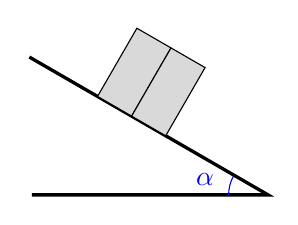
\begin{tikzpicture}
    \draw[very thick] (0,0) -- (3,0) -- ++(150:3.5cm);
    \draw[fill=gray!30,rotate around={-30:(3,0)}] (0.5,0)
    rectangle (1,1); 
    \draw[fill=gray!30,rotate around={-30:(3,0)}] (1,0) rectangle
    (1.5,1);
    \draw[blue] (2.5,0) arc (180:150:0.5cm);
    \draw (2.2,0.2) node[blue] {$\alpha$};
  \end{tikzpicture}
}
% Россия-1996, 10 класс